% THIS IS CURRENTLY A ROUGH DRAFT
% TODO:
% - Bullet points -> prose
% - Notes/random ideas jotted down -> comments
% - Figures:
%   - handle subfigures properly
%   - put captions properly into floats

\chapter{Single-cell flavin-based yeast metabolic cycles}
\label{ch:biology}

%\section{Relationship between the metabolic cycle and cell division cycle: synchrony and autonomy}

In this study, we show that yeast cells show oscillations in the fluorescence of flavins consistent with the yeast metabolic cycle.  These oscillations synchronise with the cell division cycle in permissive conditions.  Such flavin oscillations exhibited different behaviour in respiratory conditions.  Additionally, we found that cells were able to autonomously reset the phase of their metabolic cycle, independently of the cell division cycle, in response to abrupt nutrient changes.  Finally, we showed that deletion strains generated flavin oscillations that exhibited different behaviour from dissolved oxygen oscillations from chemostat conditions.

Our results confirm that the metabolic cycle is an autonomous oscillator, independent of the cell division cycle, and responds to perturbations in the environment\ldots{}

\section{Single-cell flavin oscillations synchronise with cell division cycle in permissive conditions.}
\label{sec:biology-sync}

\begin{itemize}
\item \emph{Bottom line:} We observed oscillations in the fluorescence of flavins over time from single \emph{Saccharomyces cerevisiae} cells.  For a given cell, these oscillations peak when a bud forms.  However, there were some cases in which there was an oscillation without bud formation.
\item \emph{Importance of this section:} We did this to confirm that we are looking at the yeast metabolic cycle and this is important because we use a different single-cell microfluidics setup from previous studies and we use flavin, a fluorescent compound that is less used as an indicator of the yeast metabolic cycle.  Specifically, our experiments aim to confirm the flavin oscillations described by \cite{baumgartnerFlavinbasedMetabolicCycles2018}.  In addition, we show the use of a more informative cell division cycle marker and automated identification of budding events.
\item \emph{Evidence:}
\begin{itemize}
\item Figures 1-2.
\end{itemize}

\item \textbf{Missing experiments:}
\begin{itemize}
\item Record NAD(P)H oscillations.  If possible, do it with flavin in the same cells.  If not, then compare these oscillations with the timing of birth events.  This experiment will strengthen the evidence that I am observing single-cell YMCs.  \cite{baumgartnerFlavinbasedMetabolicCycles2018} didn't do this; maybe that's why they haven't had many citations.
\item fas1\(\Delta\) to verify the role of lipids and attempt to rescue with lipid sources (e.g. glycerol trihexanoate, glycerol trioctanoate). \emph{Will start another avenue of exploration entirely, i.e. what makes up the flavin signal in a cell}
\end{itemize}
\end{itemize}

\subsection{Figure 1}
\label{sec:org6662011}
\begin{itemize}
\item \begin{center}
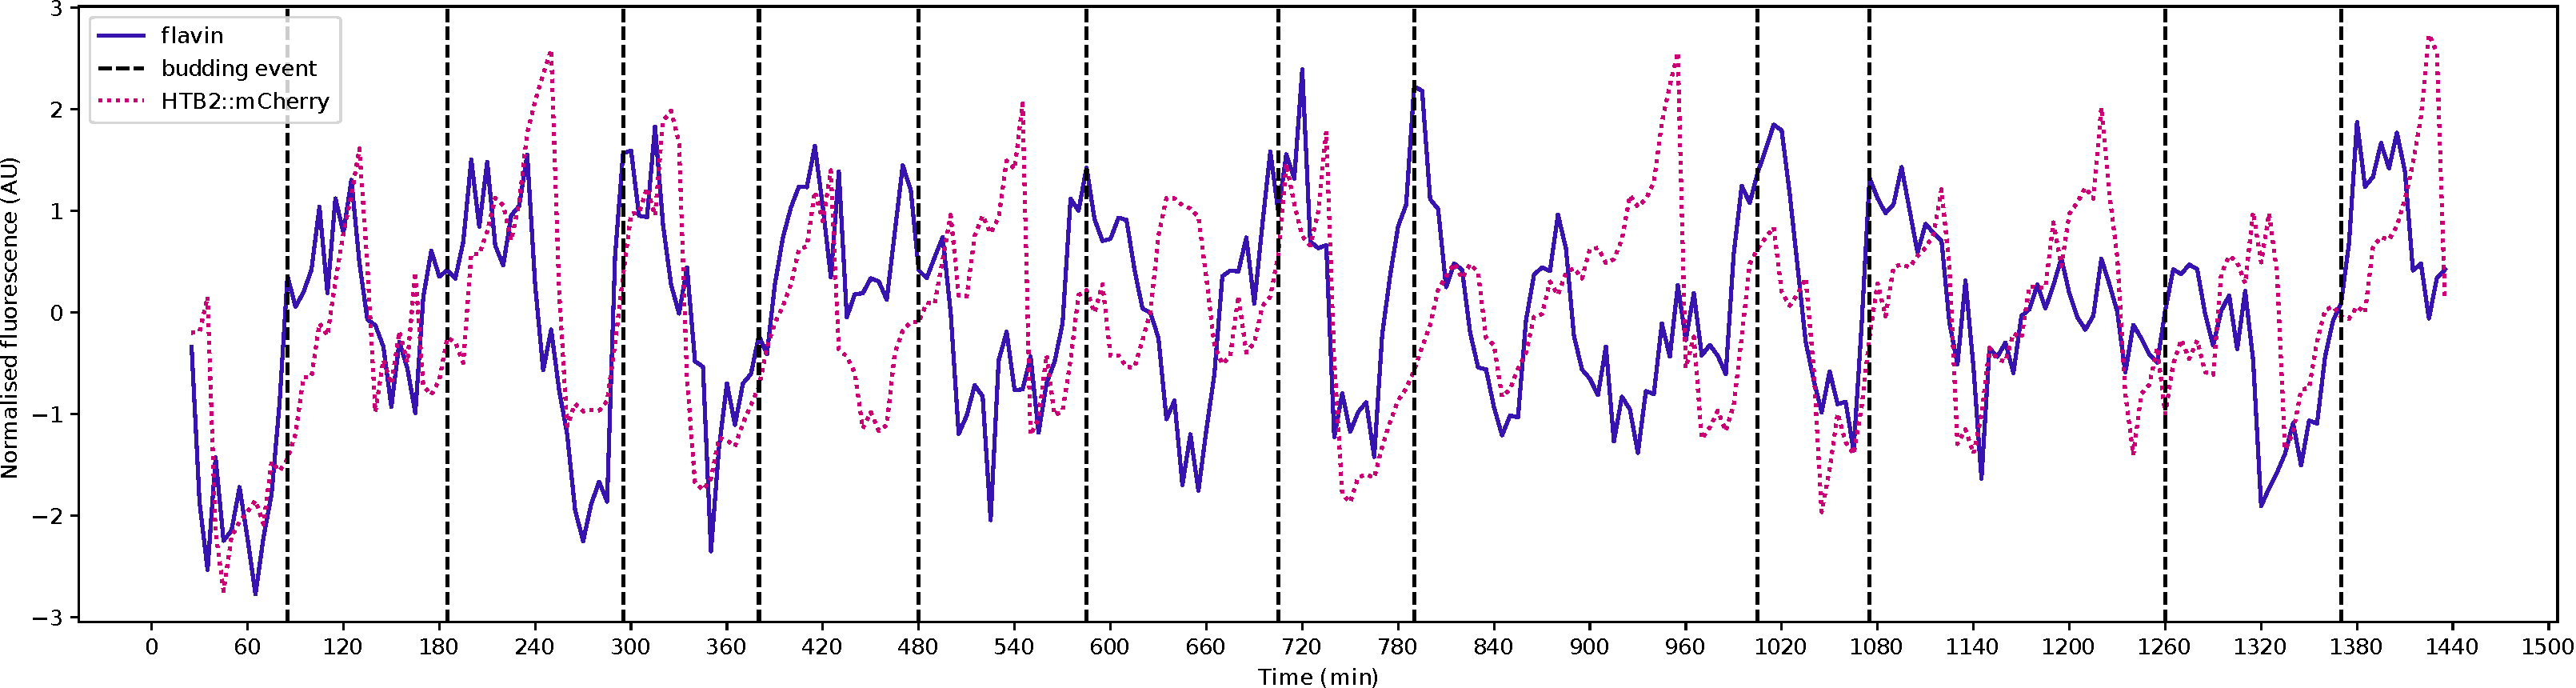
\includegraphics[width=.9\linewidth]{single_birth_plot_edit.pdf}
\end{center} Figure X: Oscillations of flavin fluorescence in the yeast metabolic cycle synchronise with events in the cell division cycle.  Figure shows sample flavin fluorescence (purple) and histone 2B (pink) level in a single cell grown in 20 g/L glucose.  Vertical dashed lines (black) indicate budding.

\begin{itemize}
\item Histone 2B levels shows phases of the cell division cycle, the most obvious being S phase and anaphase, (\cite{garmendia-torresMultipleInputsEnsure2018}) but traces are noisy.  BABY provides data that confirms timing of cell division cycle, i.e. budding times, volume and growth rate changes, cytokinesis.
\end{itemize}
\end{itemize}

\subsection{Figure 2}
\label{sec:orga6d8d36}
\begin{itemize}
\item Figure X: The yeast metabolic cycle and cell division cycle synchronise within each cell in a population of cells (n = 400) under the same conditions (20 g/L glucose).  Subfigures X-X quantify the duration of the metabolic cycle, comparative to the duration of the cell division cycle in subfigure X.

\begin{itemize}
\item \begin{center}
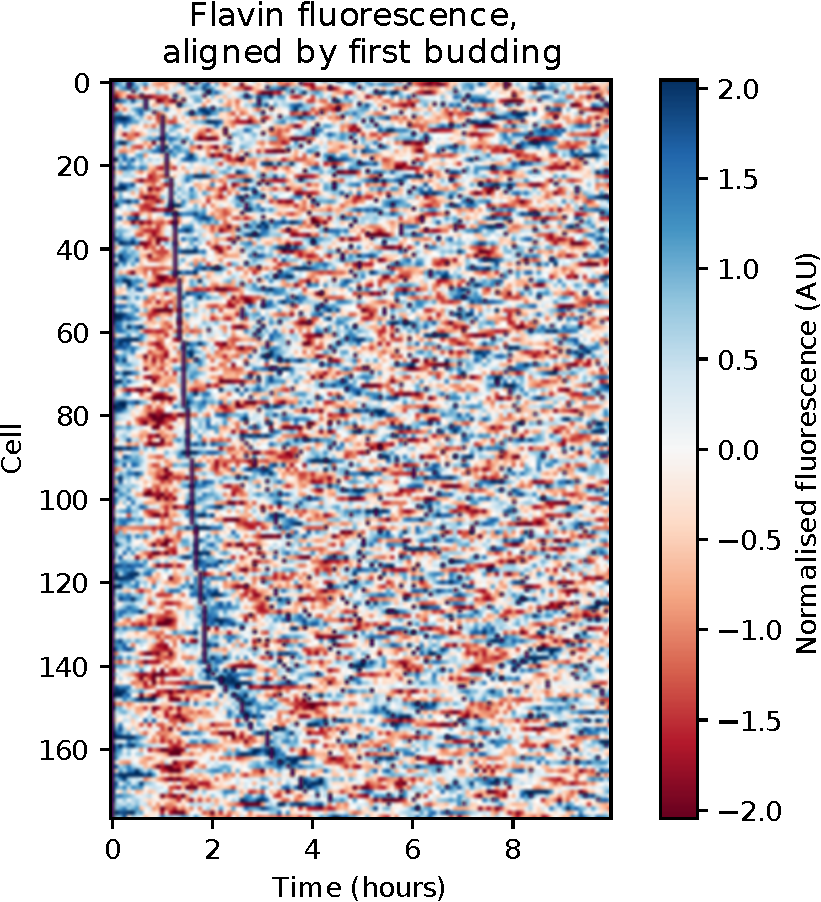
\includegraphics[width=.9\linewidth]{heatmap_edit.pdf}
\end{center} Subfigure X.1: Heatmap shows the flavin fluorescence of each cell in a population over time.  Each row of pixels represents one of 180 cells grown in 20 g/L glucose.  Fluorescence is represented as colours with red indicating low signal and blue indicating high signal.  Each budding event is indicated as a black pixel.  Flavin signals have been aligned so that the first budding event occurs at 0 hours to show that (1) budding events synchronise with peaks in fluorescence, and (2) the cell division cycle varies between cells.
\item \begin{center}
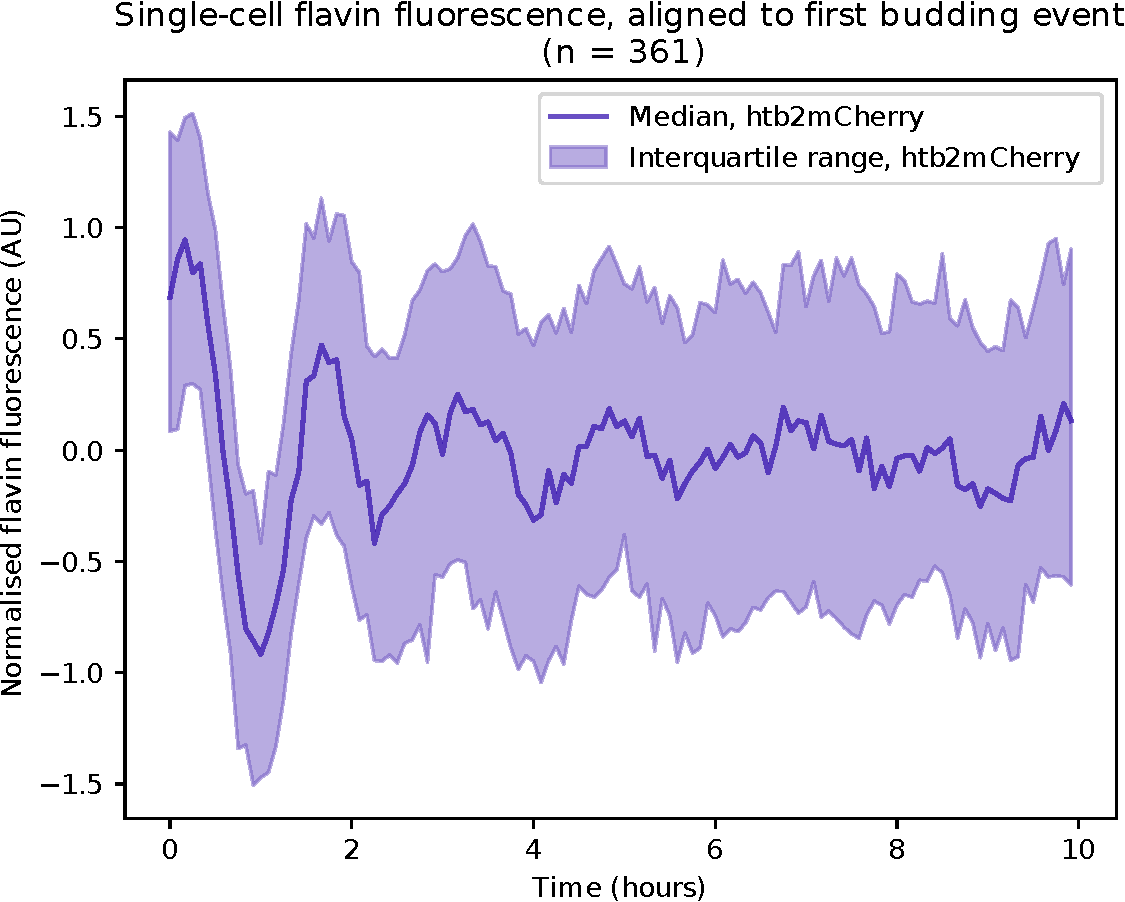
\includegraphics[width=.9\linewidth]{median_aligned_edit.pdf}
\end{center} Subfigure X.2: Median flavin fluorescence signal across cells (n = 361).  For each time point, the figure shows the median and interquartile range of the fluorescence at such time point across the population of cells.  The oscillatory shape of the median signal confirms that synchrony between flavin oscillations and cell division cycle holds across a large population of cells.
\item \begin{center}
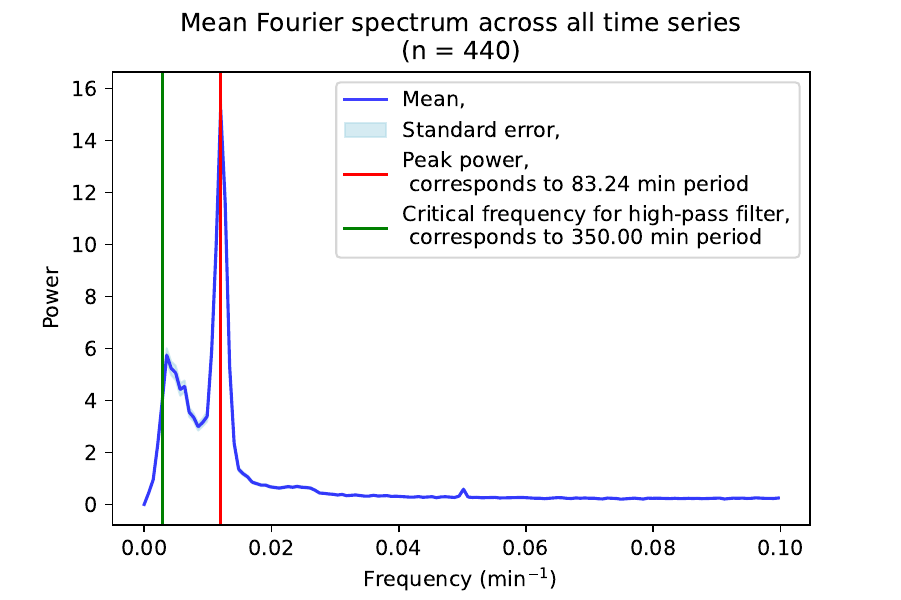
\includegraphics[width=.9\linewidth]{fy4_26643_plots_10.png}
\end{center} Subfigure X.3: Mean Fourier spectrum of flavin fluorescence across cells, indicating the duration of the metabolic cycle.  All signals were passed through a high-pass Butterworth filter with a critical frequency of 1/350 min\textsuperscript{-1} to remove long-term trends to reveal oscillatory behaviour; see methods.
\item \begin{center}
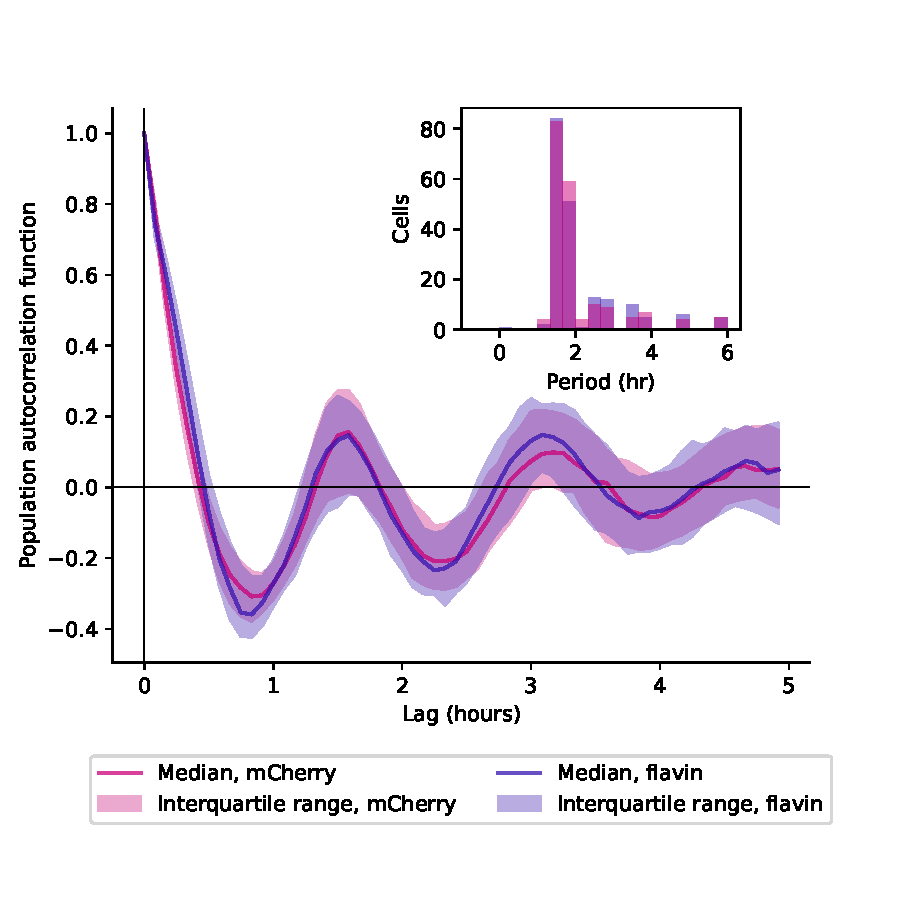
\includegraphics[width=.9\linewidth]{acf_and_histogram.pdf}
\end{center} Subfigure X.4: \textbf{(Main)} Median autocorrelation functions and interquartile ranges of flavin fluorescence (purple) and histone 2B levels (pink) across population of cells, along with \textbf{(inset)} the distribution of the periods of each oscillator across cells as determined by the strongest frequency in each signal's Fourier spectrum.  This figure indicates that the cells' metabolic cycles and cell division cycles are both consistently 90 minutes long.
\end{itemize}

\begin{itemize}
\item \begin{center}
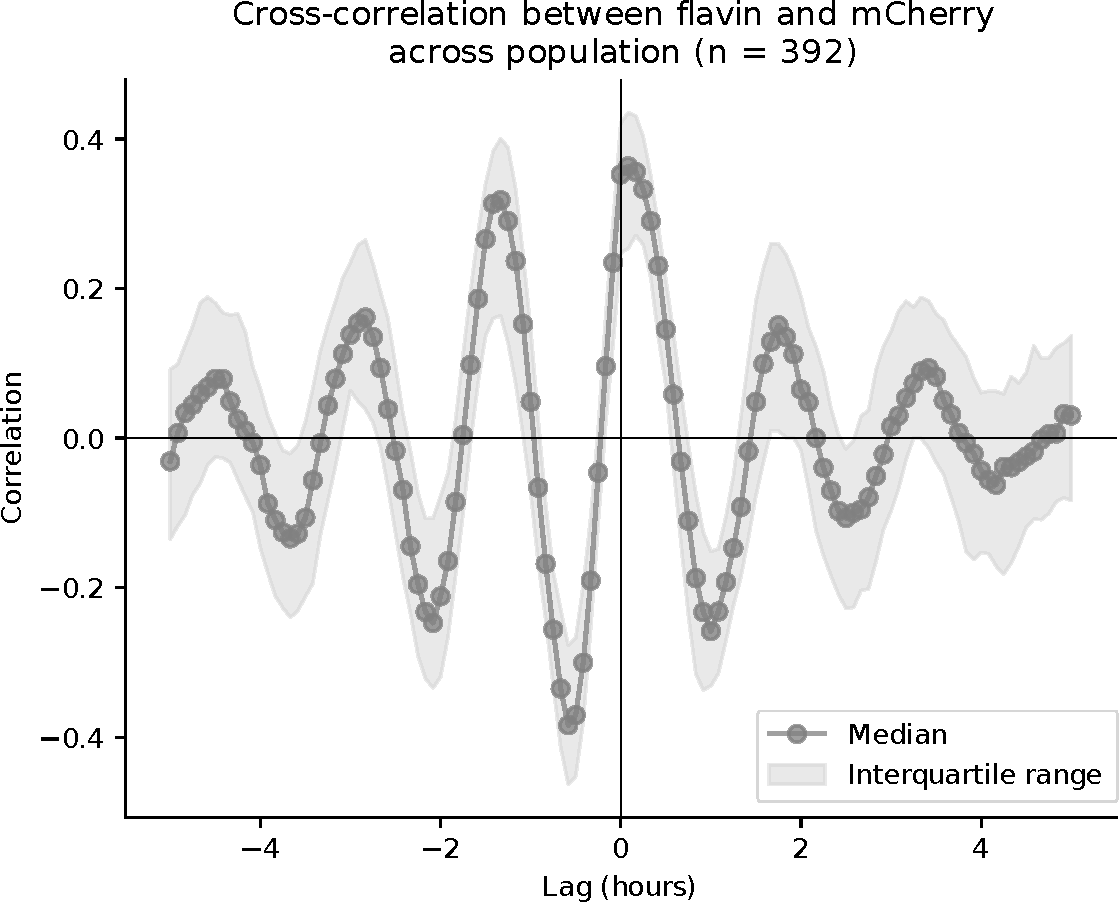
\includegraphics[width=.9\linewidth]{xcf_edit.pdf}
\end{center} Subfigure X.X: Cross-correlation between flavin and histone 2B signals (n = 392), indicating that histone levels peak 5 minutes after flavin fluorescence peaks.
\end{itemize}
\end{itemize}


\section{Cells autonomously generate flavin oscillations, independently of the cell division cycle, in response to abrupt nutrient changes.}
\label{sec:biology-abrupt}

\begin{itemize}
\item \emph{Bottom line:} We found that when cells grown in high (7.5 g/L) glucose were abruptly starved of glucose, their flavin oscillations reset phase.  These flavin oscillations under starvation continue without budding events or with sparse budding events.
\item \emph{Importance of this section:}

\begin{itemize}
\item Many chemostat-based studies (citations needed) along with a modelling study (\cite{krishnaMinimalPushPull2018}) suggest that a diffusible metabolite is responsible for the synchrony of the metabolic cycle across cells, while single-cell studies suggest that cells independently generate these oscillations.  I aim to confirm the conclusions from \cite{papagiannakisAutonomousMetabolicOscillations2017}, but in flavin.
\end{itemize}
\item \emph{Evidence:}
\begin{itemize}
\item Figure 3.
\item When cells are in high glucose, oscillations are asynchronous (confirms \cite{papagiannakisAutonomousMetabolicOscillations2017,baumgartnerFlavinbasedMetabolicCycles2018}).
\end{itemize}

\item \textbf{Missing experiments:}
\begin{itemize}
\item Adding acetate, acetaldehyde, or ethanol in bulk.  See if it synchronises YMCs, as described in chemostats by \cite{kuangMsn2RegulateExpression2017} and \cite{krishnaMinimalPushPull2018} .  If so, this would start a discussion about what processes trigger resetting YMC phases and their biological explanations.
\item Feast-and-famine, or glucose pulsing (\cite{charvinForcedPeriodicExpression2009}).
\end{itemize}
\item \textbf{Missing discussion:}
\begin{itemize}
\item I observed no/weaker synchrony of oscillations between cells if the cells were grown in 10 g/L glucose.  Perhaps we can spin this as a result.  In any case, we need supplementary information to justify 7.5 g/L glucose when I used 20 g/L earlier.  This information can be Monod's Law experiments (e.g. by Hongpei) that suggests that 7.5 g/L is past saturation.
\end{itemize}
\end{itemize}

\subsection{Figure 3}
\label{sec:org9b50c2e}
\begin{itemize}
\item Figure X: Metabolic cycles between physically separate cells synchronise upon abrupt starvation.  Cells were grown in 7.5 g/L glucose for 7 hours before being abruptly switched to 0 g/L glucose for 8 hours and then resumed to 7.5 g/L glucose for 7 hours.
\begin{itemize}
\item \begin{center}
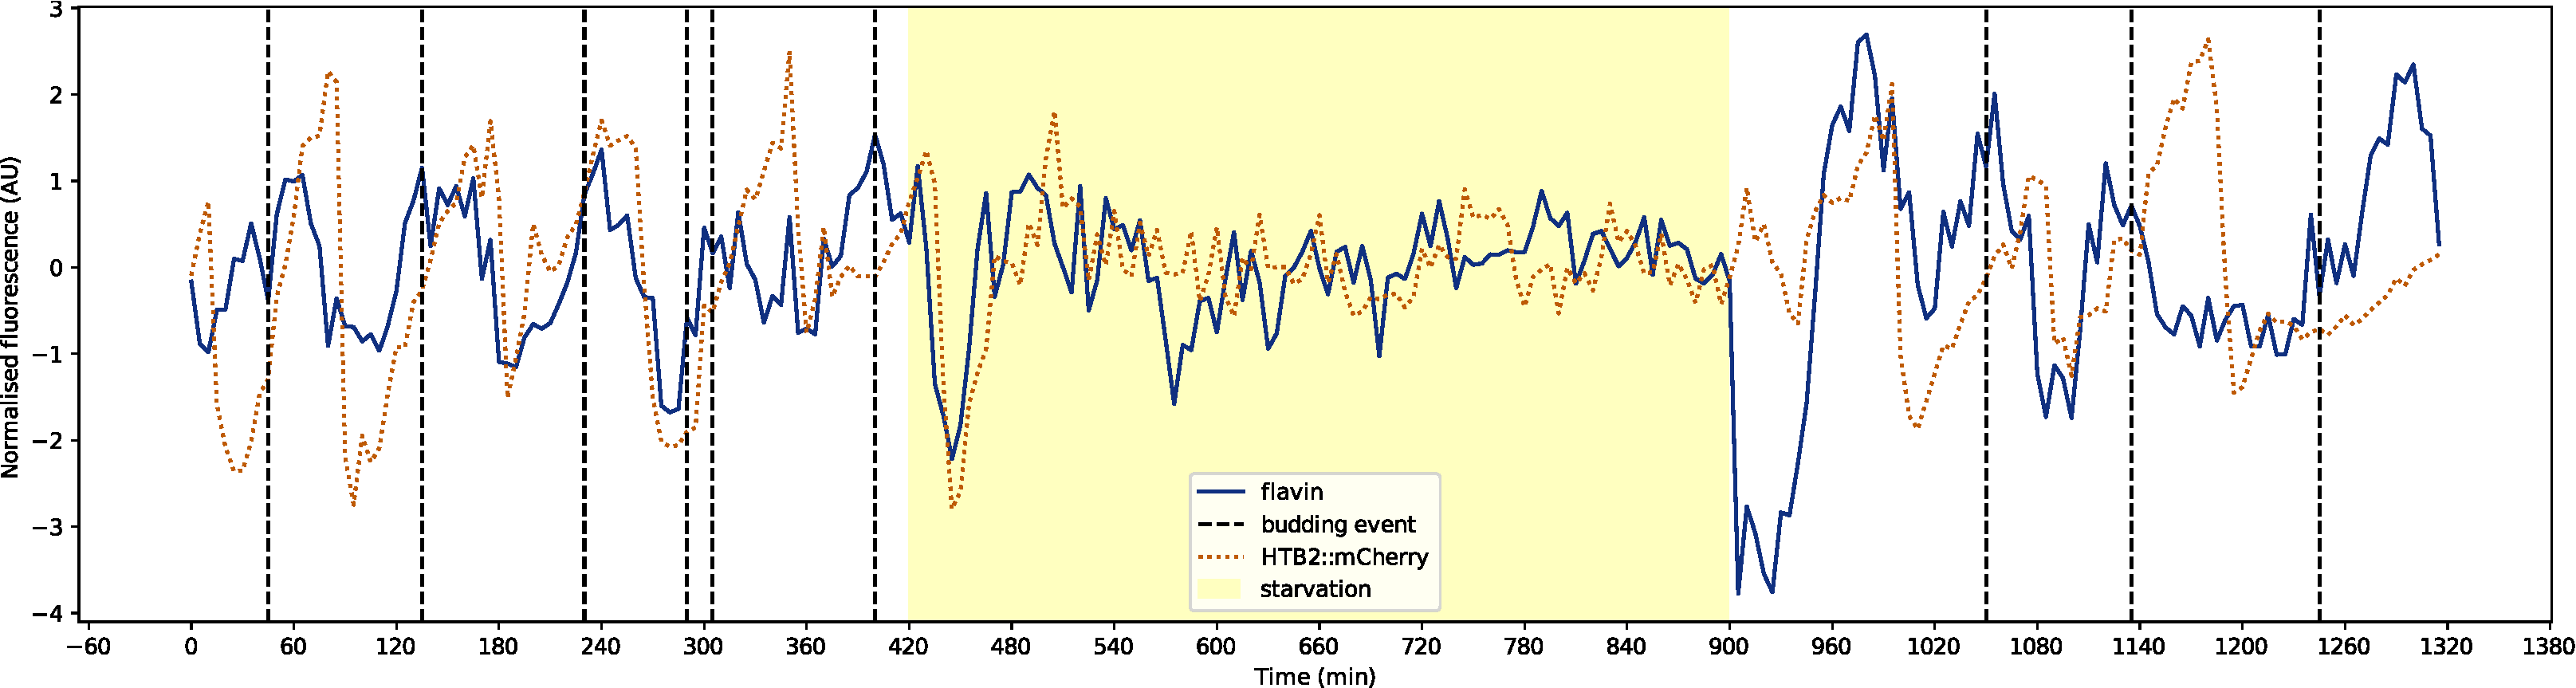
\includegraphics[width=.9\linewidth]{starvation_single_birth_plot_new_edit.pdf}
\end{center} Subfigure X.X: Flavin fluorescence synchronises with the cell division cycle in high-glucose conditions before and after starvation.  Figure shows sample flavin fluorescence levels (purple) and histone 2B localisation (pink) in single cells.  Vertical lines (black) indicate budding.
\end{itemize}
\end{itemize}

\begin{itemize}
\item \begin{center}
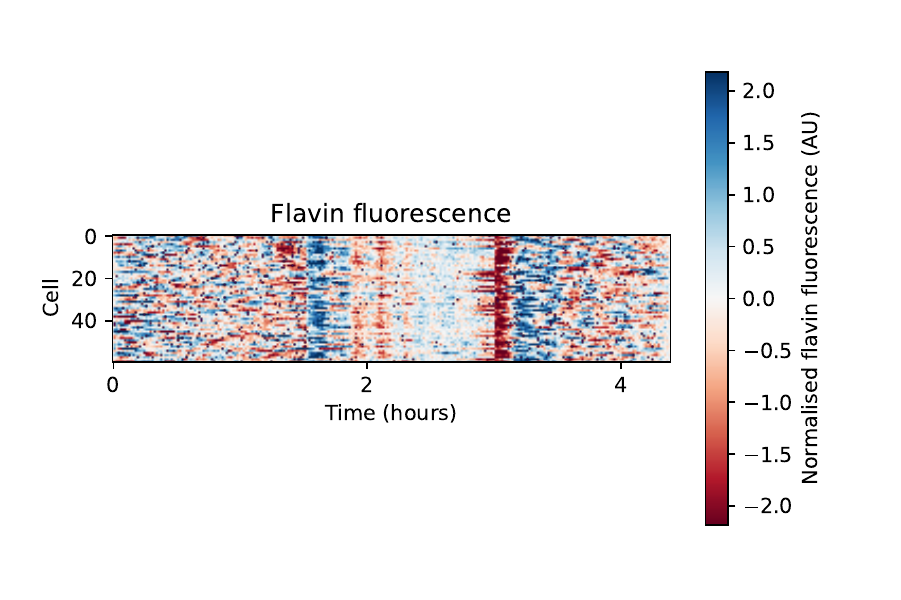
\includegraphics[width=.9\linewidth]{fy4_19972_plots_butter_04.png}
\end{center} Subfigure X.X: Heatmap shows the flavin fluorescence of each cell in a population over time.  Each row of pixels represents one of 60 cells.  Fluorescence is represented as colours with blue indicating low signal and red indicating high signal.  Each budding event is indicated as a black pixel.  This figure additionally shows that budding events were sparse during starvation.
\end{itemize}


\section{Effect of carbon source on YMC.}
\label{sec:biology-carbon}

\begin{itemize}
\item \emph{Bottom line:} We found that\ldots{}
\begin{itemize}
\item When the cells were grown in a non-fermentable carbon source (20 g/L sodium pyruvate), the cells showed longer metabolic cycles and cell division cycles.  Though the longer cell division cycles were because of longer G1 phases but unchanged S/M phases.  Furthermore, the synchrony between the two oscillators remain, but there were more cases in which the flavin signal peaks without a budding event \textbf{(supplementary figures)}
\begin{itemize}
\item (Add statistical tests to reject the null hypothesis that the mean duration of metabolic cycles in pyruvate is equal to the mean duration of metabolic cycles in high glucose.)
\end{itemize}
\item When the cells were grown in limiting glucose that emulates conditions in a chemostat (10 mg/L glucose), the cells showed longer metabolic cycles and an absence of cell division.  Furthermore, the signals are of low amplitude and low quality, as evidenced by the low signal-to-noise ratios.
\begin{itemize}
\item (Add statistical tests to reject the null hypothesis that the distribution of SNRs are the same between the three nutrient conditions.)
\end{itemize}
\item In contrast to 20 g/L glucose in which metabolic cycles were asynchronous, in these conditions there is some degree of metabolic cycle synchrony between cells. \textbf{(add figures)}
\end{itemize}
\item \emph{Importance of this section:}
\begin{itemize}
\item Confirm \cite{papagiannakisAutonomousMetabolicOscillations2017} but in flavin, extend in more carbon sources.  It is known that nutrient changes affect the YMC (citation needed).
\item Limiting carbon sources emulate the chemostat.
\end{itemize}
\item \emph{Evidence:}
\begin{itemize}
\item Figures 4-5.
\end{itemize}

\item \textbf{Missing experiments:}
\begin{itemize}
\item Raffinose.  This is a carbon source that \cite{papagiannakisAutonomousMetabolicOscillations2017} did not use.  It is a trisaccharide and a common non-glucose pre-growth carbon source, certainly in Hxt- and sugar-related studies (Yu).  Yeast must secrete invertase to metabolise it and metabolism on this compound is slow.  So, growth on raffinose emulates a low-glucose concentration and the cell respires.  However, there is a risk that invertase is washed away in microfluidic experiments, so the growth rate should be tested first before subsequent experiments.
\end{itemize}
\end{itemize}

\subsection{Figure 4}
\label{sec:orgf8ff501}
\begin{itemize}
\item Figure X: When cultivated in 20 g/L pyruvate, cells show longer metabolic cycles while the S/M phase of the cell division cycle remains the same length and the G1 phase lengthens.
\begin{itemize}
\item \begin{center}
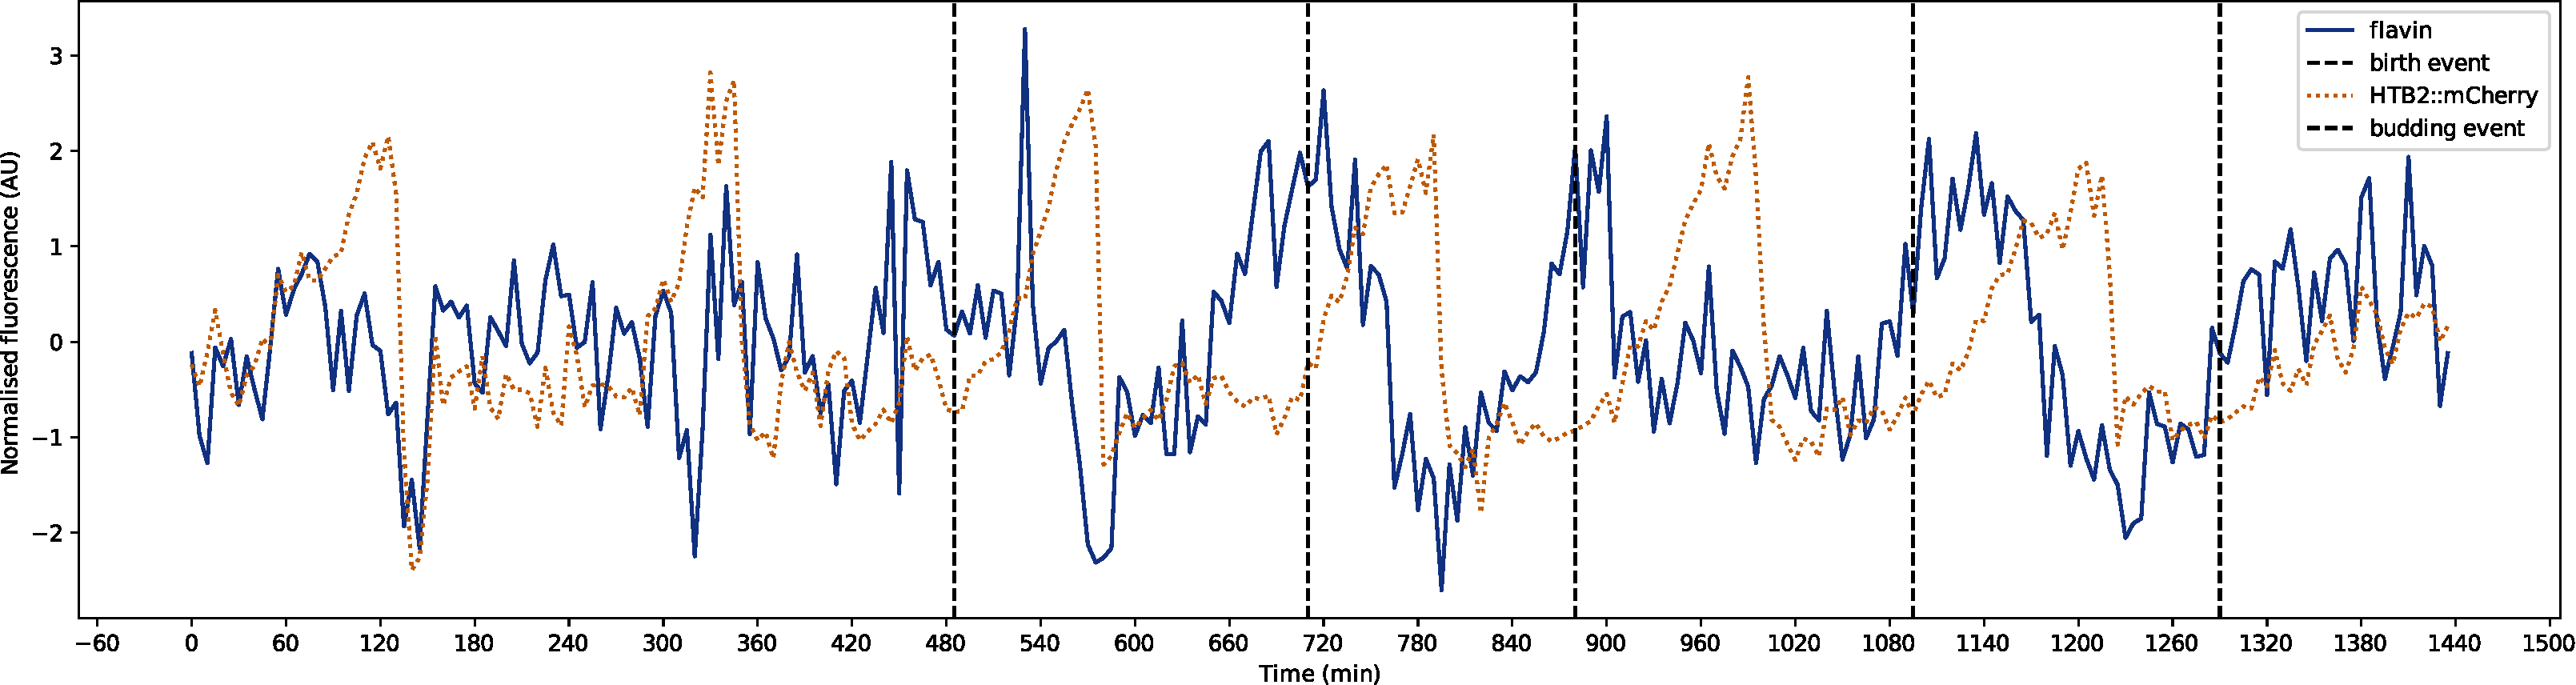
\includegraphics[width=.9\linewidth]{pyruvate_single_birth_plot_edit.pdf}
\end{center} Subfigure X.X: Oscillations of flavin fluorescence lengthen when cells are cultivated in pyruvate while the duration of S/M phase stays constant.  Figure shows sample flavin fluorescence (purple) and histone 2B (pink) level in a single cell grown in 20 g/L pyruvate.  Vertical dashed lines (black) indicate budding.
\end{itemize}

\begin{itemize}
\item \begin{center}
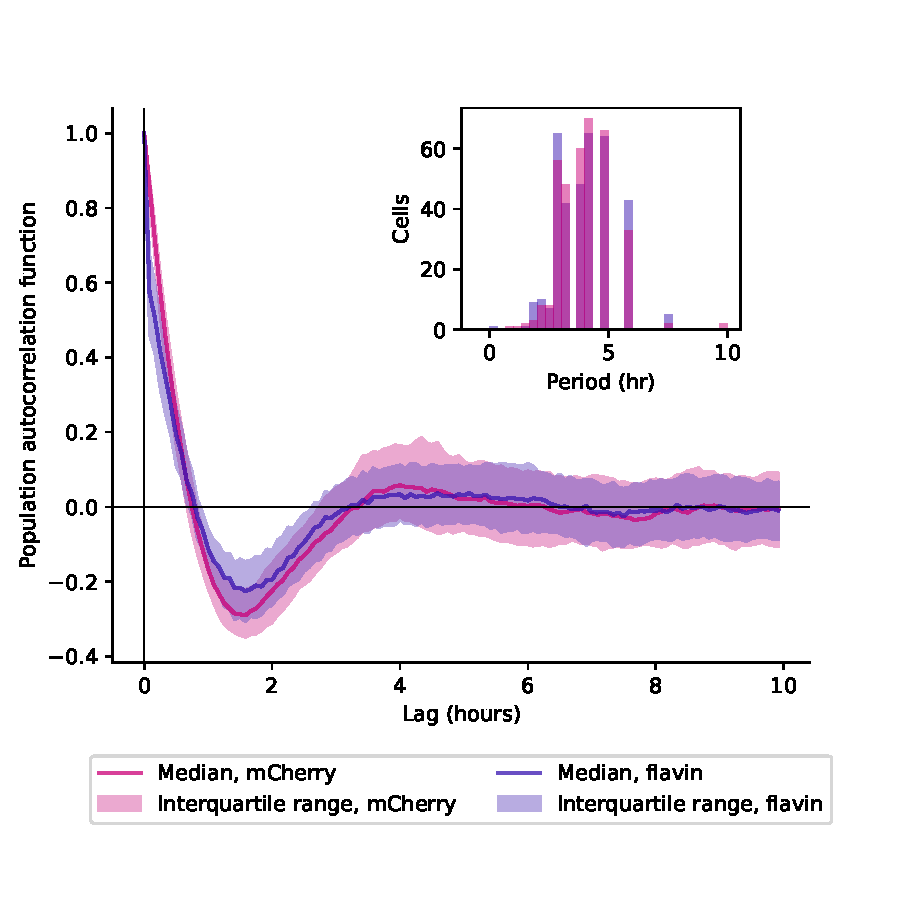
\includegraphics[width=.9\linewidth]{pyruvate_acf_and_histogram.pdf}
\end{center} Subfigure X.X: \textbf{(Main)} Median autocorrelation functions and interquartile ranges of flavin fluorescence (purple) and histone 2B levels (pink) across population of cells, along with \textbf{(inset)} the distribution of the periods of each oscillator across cells as determined by the strongest frequency in each signal's Fourier spectrum.  This figure indicates that the cells' metabolic cycles and cell division cycles are both consistently approximately 4 hours long.
\end{itemize}

\begin{itemize}
\item \begin{center}
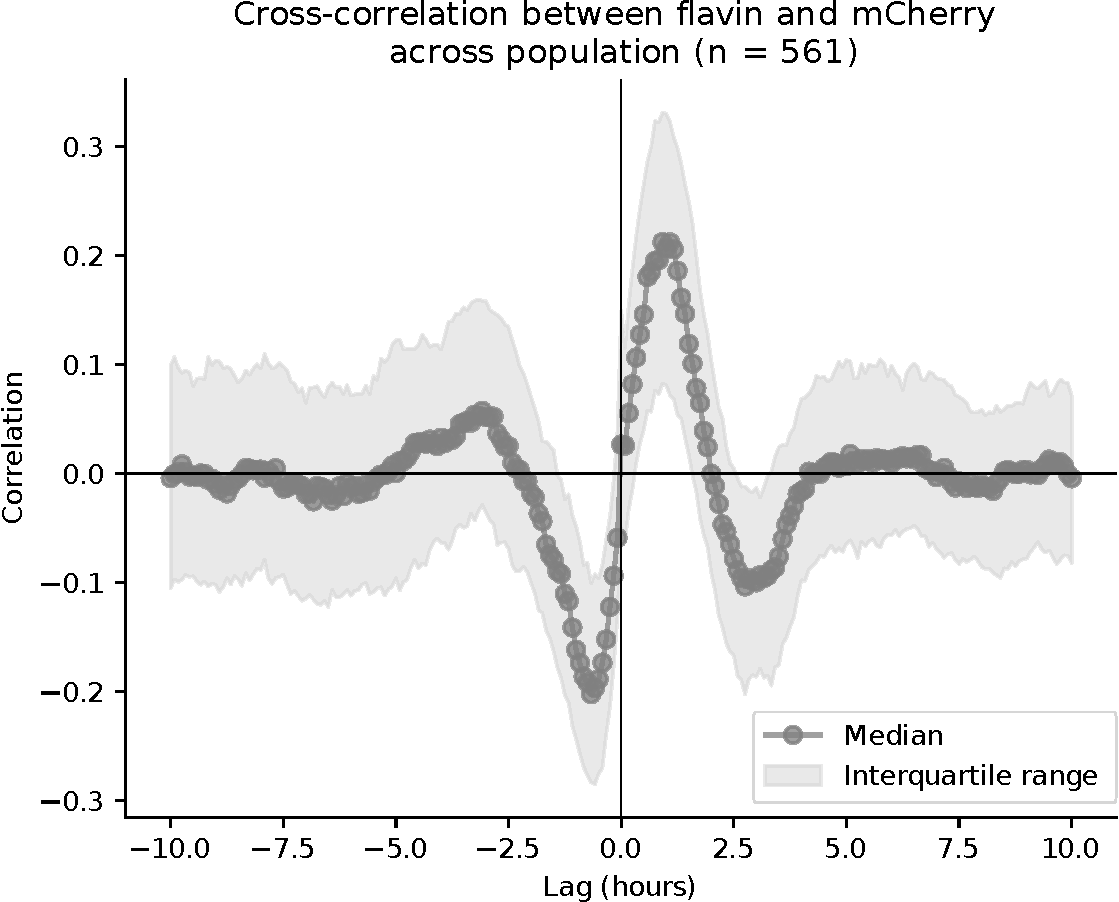
\includegraphics[width=.9\linewidth]{pyruvate_xcf_edit.pdf}
\end{center} Subfigure X.X: Cross-correlation between flavin and histone 2B signals (n = 561), indicating that histone levels peak 1 hour after flavin fluorescence peaks.
\end{itemize}
\end{itemize}

\subsection{Figure 5}
\label{sec:org16a2ef0}
\begin{itemize}
\item Figure X: When cultivated in growth-limiting (10 mg/L) glucose, cells show lower-quality metabolic cycles with lower amplitudes.

\begin{itemize}
\item \begin{center}
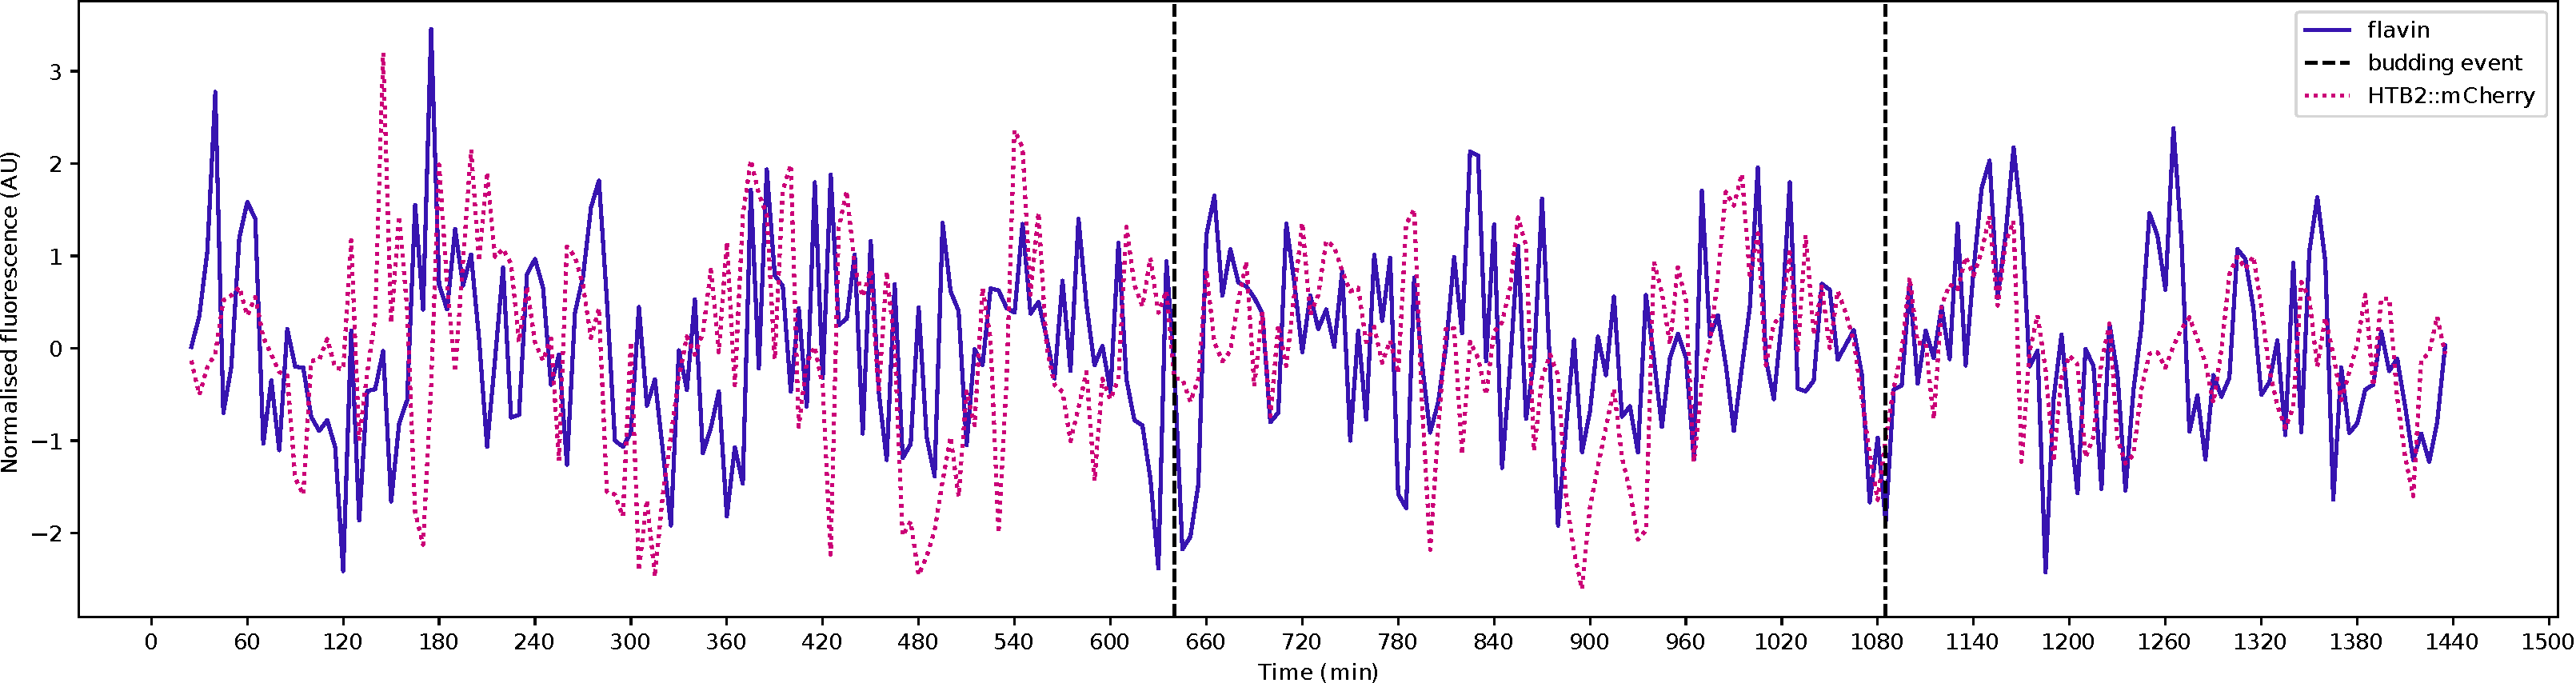
\includegraphics[width=.9\linewidth]{limiting_single_birth_plot_edit.pdf}
\end{center} Subfigure X.X: Oscillations of flavin fluorescence are noisier when cells are cultivated in 10 mg/L glucose while cells do not show growth and division.  Figure shows sample flavin fluorescence (purple) and histone 2B (pink) level in a single cell grown in 10 mg/L glucose.  Vertical dashed lines (black) indicate budding.
\item \begin{center}
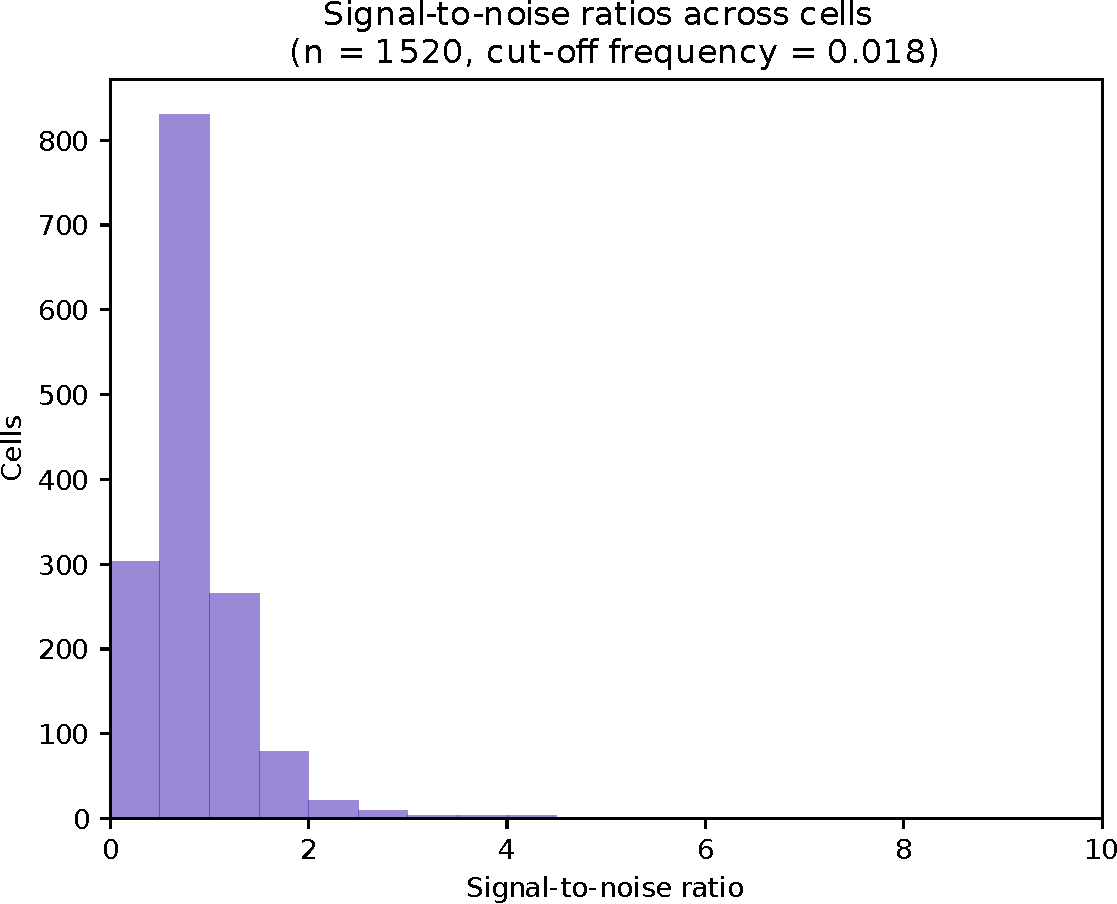
\includegraphics[width=.9\linewidth]{limiting_snr_edit.pdf}
\end{center} Subfigure X.X: Distribution of signal-to-noise ratios computed for each flavin time series derived from cells cultivated in 10 mg/L glucose, showing that most cells have noisy signals and thus implying low-amplitude metabolic cycles.  Fourier spectra were computed for each cell's flavin time series and a cut-off frequency is defined; the signal-to-noise ratio is defined as the area under the spectrum to the left (lower frequencies, representing signal) of the cut-off divided by the area to the right (higher frequencies, representing noise).
\item \begin{center}
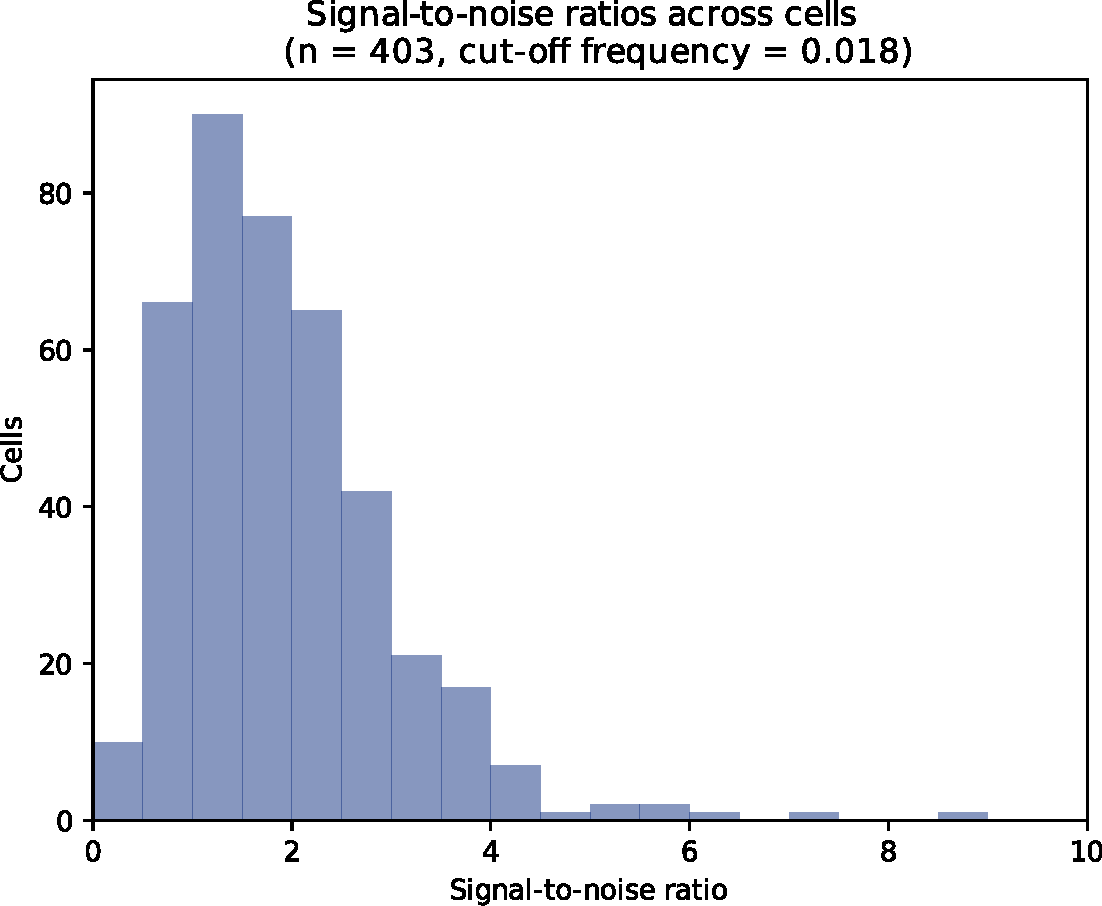
\includegraphics[width=.9\linewidth]{pyruvate_snr_edit.pdf}
\end{center} Subfigure X.X: Distribution of signal-to-noise ratios computed for each flavin time series derived from cells cultivated in 20 g/L pyruvate, showing that cells have higher-quality signals.
\item \begin{center}
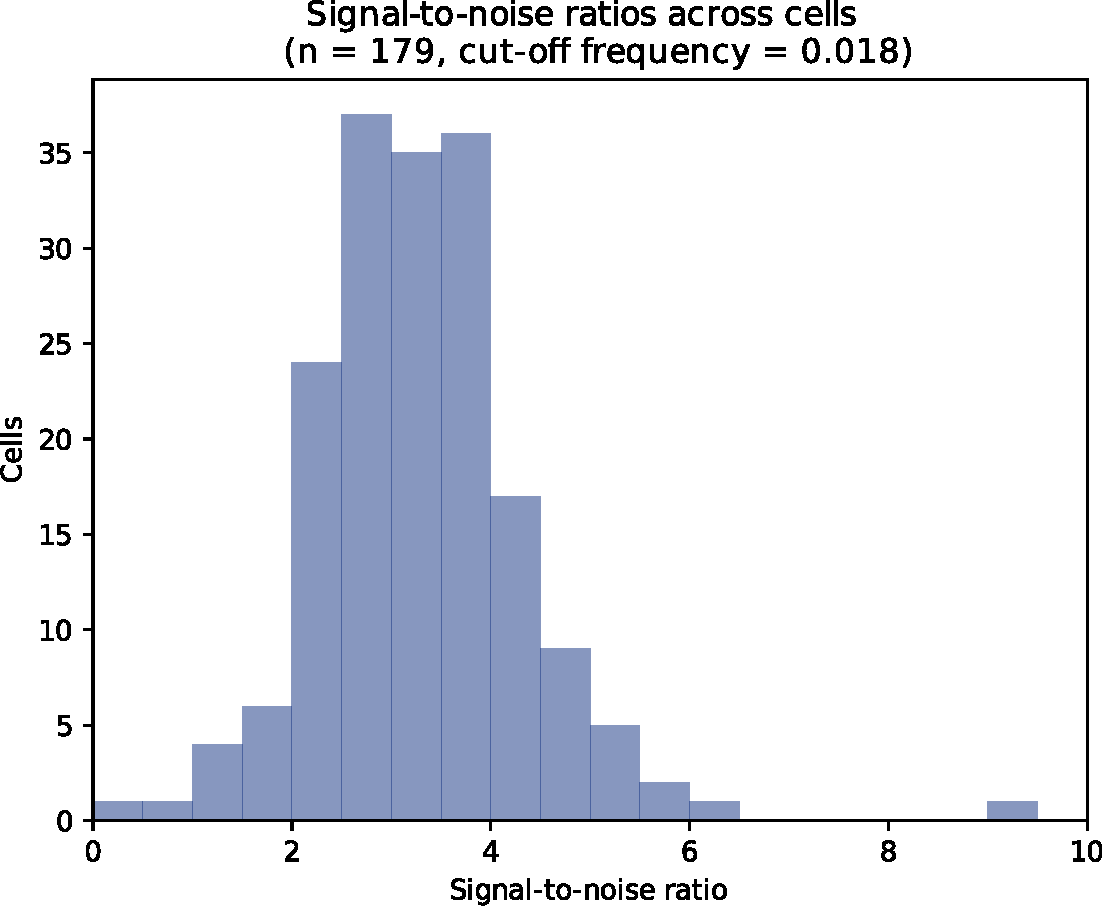
\includegraphics[width=.9\linewidth]{glucose_snr_edit.pdf}
\end{center} Subfigure X.X: Distribution of signal-to-noise ratios computed for each flavin time series derived from cells cultivated in 20 g/L glucose, showing that cells have high-quality signals.
\end{itemize}
\end{itemize}


\section{Do single-cell flavin traces recapitulate dissolved-oxygen YMCs in chemostats, particularly in deletion strains?}
\label{sec:biology-deletions}

\begin{itemize}
\item \emph{Bottom line:} We found that\ldots{}
\begin{itemize}
\item Single-cell metabolic oscillations are not reliably generated from the auxotrophic zwf1\(\Delta\) strain, which has been shown to not generate dissolved-oxygen oscillations in the chemostat (\cite{tuCyclicChangesMetabolic2007}).
\item Single-cell metabolic oscillations are also not reliably generated from the auxotrophic tsa1\(\Delta\) tsa2\(\Delta\) strain, which has been generate dissolved-oxygen chemostat oscillations of a different waveform as the wild type strain (\cite{caustonMetabolicCyclesYeast2015}).  I also observe cells getting sick, i.e.\ bloating and clogging earlier than the wild type.
\item Single-cell metabolic oscillations are generated by certain prototrophic deletion strains (swe1\(\Delta\), rim11\(\Delta\), and tsa1\(\Delta\) tsa2\(\Delta\)) and have properties that differ from wild-type.  However, these differences do not reflect how dissolved-oxygen oscillations differ from their wild-type equivalents (\cite{caustonMetabolicCyclesYeast2015}).
\end{itemize}
\item \emph{Importance of this section:}
\begin{itemize}
\item Attempt to show that the single-cell metabolic cycle and the chemostat metabolic cycle are the same cycle.
\item Chemostat experiments obscure the behaviour of individual cells.  My experiments should produce a more detailed picture of how changes to the metabolic cycle affect the coarse-grained readouts in chemostat-based studies.
\item With deletion strains, I can give some mechanistic insight on YMC, otherwise largely unknown.
\begin{itemize}
\item \cite{tuCyclicChangesMetabolic2007}
\begin{itemize}
\item zwf1\(\Delta\): metabolic cycles abolished, key metabolic enzyme that catalyses production of NADPH, which is a key player in YMC (though other enzymes can compensate NADPH production).
\end{itemize}
\item \cite{caustonMetabolicCyclesYeast2015}
\begin{itemize}
\item swe1\(\Delta\): gene responsible for CDC processes (another biological rhythm) e.g. DNA repair.  Deletion shown to affect CDC-YMC coupling.
\item rim11\(\Delta\): gene involved in circadian rhythm (another biological rhythm).  Deletion strain shown to have shorter YMCs.
\item tsa1\(\Delta\) tsa2\(\Delta\): gene involved in redox metabolism (key player of metabolic cycle), linked to circadian rhythm (another biological rhythm).  Deletion strain shown to have shorter YMCs and of a different waveform, i.e. an additional 'dip' in dissolved oxygen corresponding to the reductive-charging phase.
\end{itemize}
\end{itemize}
\end{itemize}
\item \emph{Evidence:}
\begin{itemize}
\item Figures 6-10.
\item We include high-glucose to be consistent with my previous section.  Also including limiting glucose as it approximates chemostat conditions (\cite{jonesCyberneticModelGrowth1999}, and add other citations that say that chemostat is starvation).  If chemostat conditions mean starvation, I should look at microfluidic conditions that mimic that best.
\item Precultured in pyruvate because zwf1\(\Delta\) doesn't grow well on high glucose liquid culture (add evidence in the form of growth rate graphs), and tsa1\(\Delta\) tsa2\(\Delta\) follows for consistency.  Different amino acid formulation for BY4742 vs BY4741 because different auxotrophy.
\item The properties of the single-cell metabolic cycles we observe in Causton's strains differ from the properties of chemostat cycles \cite{caustonMetabolicCyclesYeast2015} describe.  Under starvation, the super-long CDCs suggested by chemostat studies are possible (citations needed).  However, the period of the metabolic cycles I observe are much shorter than chemostat-based metabolic cycles.  Furthermore, the shape of the metabolic cycles is different -- notably tsa1\(\Delta\) tsa2\(\Delta\) that doesn't show a 'notch' as \cite{caustonMetabolicCyclesYeast2015} showed.
\end{itemize}

\item \textbf{Missing analysis:}
\begin{itemize}
\item Sub-populations, i.e. are there sub-populations that behave differently?  It seems like at least there is a group of cells that produce just noise and a group of cells that produce long-period oscillations, and these oscillations occur over a larger spread of periods than the wild-type -- I have done some analysis that could show the latter.  This model looks likely for zwf\(\Delta\) judging by the signal-to-noise ratio histogram.  This is where time series featurisation and clustering (hierarchical, UMAP, etc.) may be useful.  But are there methods that don't rely on machine learning -- consult notes with Andrew Millar.
\item A supplementary figure should try to show equivalence between FY4 and CEN.PK (and BY4741).  There should be an experiment in which I put FY4 and CEN.PK in the same conditions. \cite{baumgartnerFlavinbasedMetabolicCycles2018} state that the two strains have equivalent metabolic cycles, so there is some precedent, but they didn't do a direct comparison.
\end{itemize}
\item \textbf{Missing experiments:}
\begin{itemize}
\item zwf1\(\Delta\) in low glucose.  Problem: auxotrophic.  Need to engineer a deletion in CEN.PK, likely with CRISPR.
\item Chemostat/turbidostat.  But we lack the expertise, and this is its own avenue entirely.  Chemostat vs single-cell equivalence can be its own PhD project.
\end{itemize}
\end{itemize}


\subsection{Figure 6}
\label{sec:org35a4444}
\begin{itemize}
\item Figure X: zwf1\(\Delta\) (BY4741) cells in high (10 g/L) glucose do not robustly generate metabolic oscillations.

\begin{itemize}
\item \begin{center}
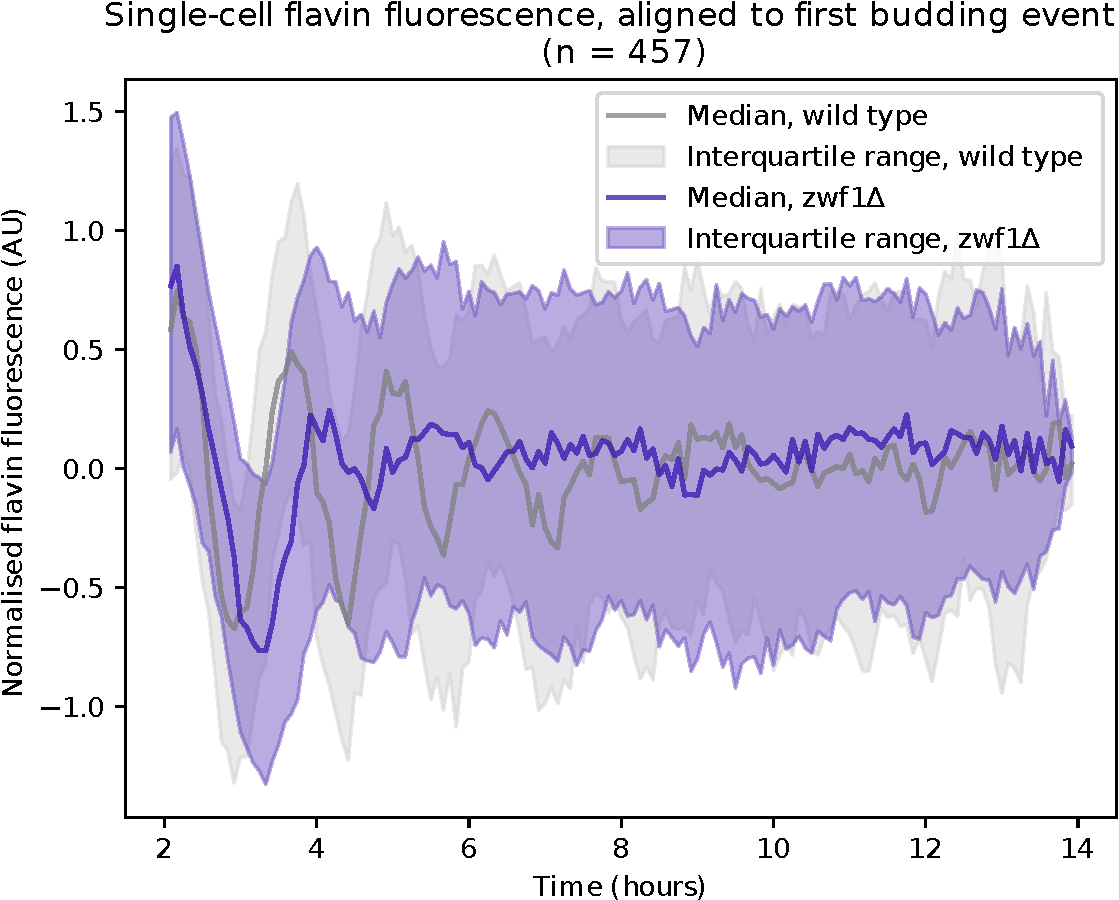
\includegraphics[width=.9\linewidth]{zwf1_align_edit.pdf}
\end{center} Subfigure X.X: Median flavin fluorescence signal across cells (n = 457); each data point is the median of flavin fluorescence at each time point relative to the first birth.  The shape of the median signal suggests that the flavin oscillations in this deletion strain do not synchronise with the cell division cycle at a uniform frequency, in contrast to its BY4741 parental strain.
\end{itemize}

\begin{itemize}
\item \begin{center}
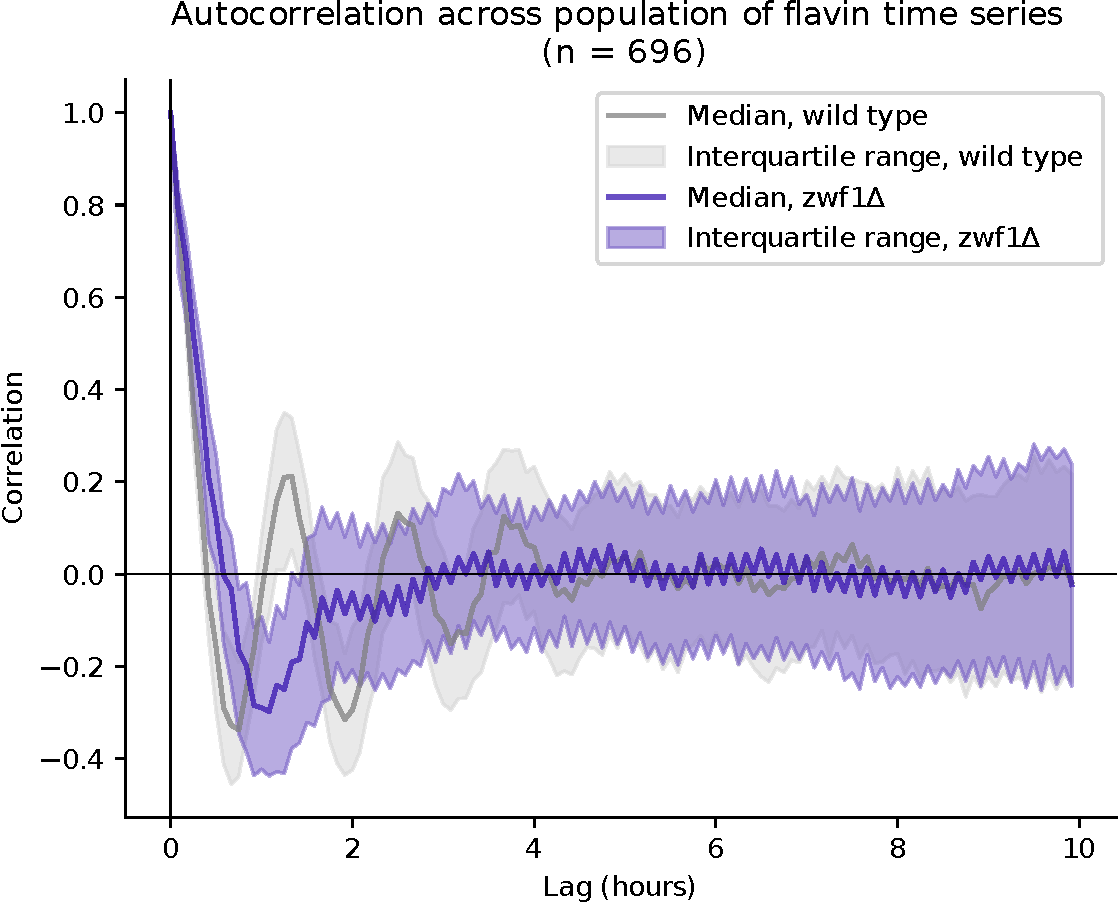
\includegraphics[width=.9\linewidth]{zwf1_acf_edit.pdf}
\end{center} Subfigure X.X: Autocorrelation function of flavin fluorescence across cells, confirms a lack of robust oscillations across the population of cells.
\item \begin{center}
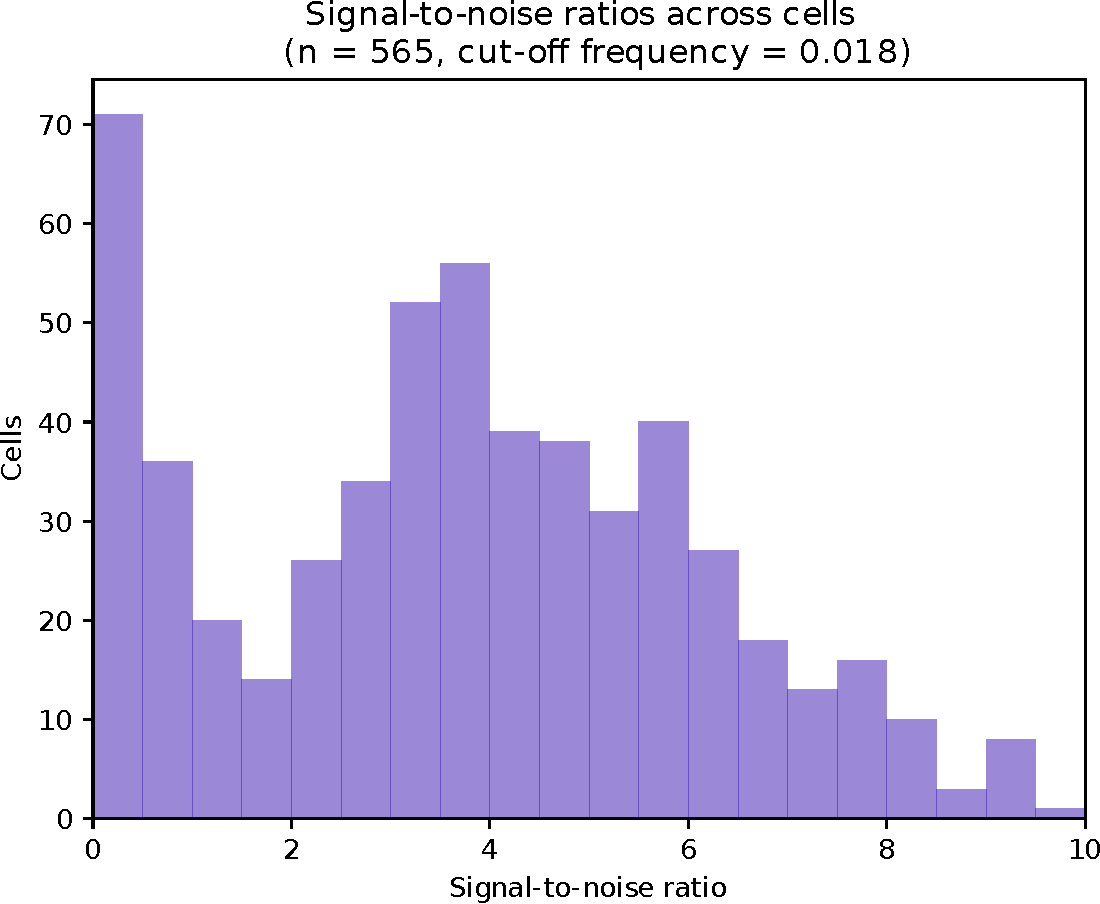
\includegraphics[width=.9\linewidth]{zwf1_snr_edit.pdf}
\end{center} Subfigure X.X: Distribution of signal-to-noise ratios computed for each flavin time series derived from zwf1\(\Delta\) cells, showing a wide distribution of quality of oscillation.
\end{itemize}
\end{itemize}


\subsection{Figure 7}
\begin{itemize}
\item Figure X: tsa1\(\Delta\) tsa2\(\Delta\) (BY4742) cells in high (10 g/L) glucose do not robustly generate metabolic oscillations.

\begin{itemize}
\item \begin{center}
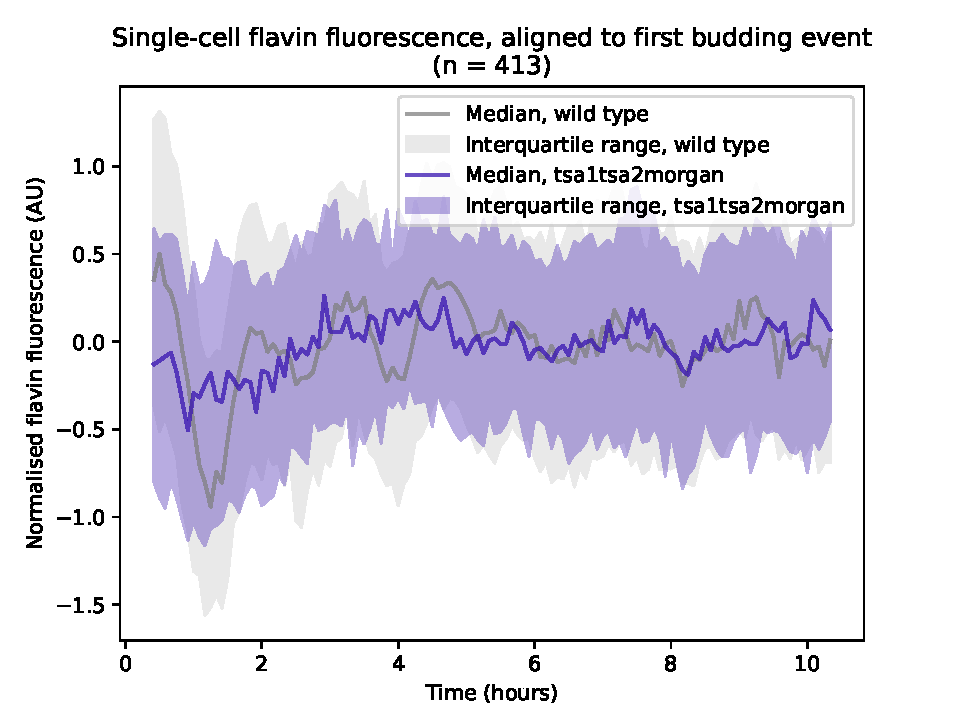
\includegraphics[width=.9\linewidth]{tsa1tsa2morgan_1253_plots_6.pdf}
\end{center} Subfigure X.X: Median flavin fluorescence signal across cells (n = 413); each data point is the median of flavin fluorescence at each time point relative to the first birth.  The shape of the median signal suggests that the flavin oscillations in this deletion strain synchronise with the cell division cycle at a slower frequency, in contrast to its BY4742 parental strain.
\end{itemize}

\begin{itemize}
\item \begin{center}
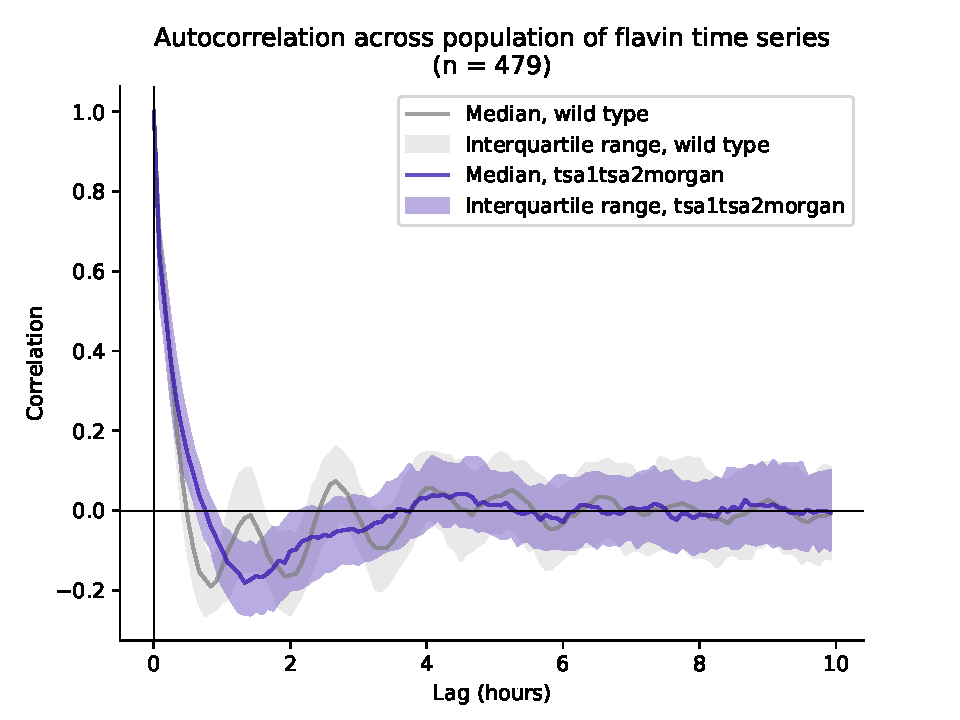
\includegraphics[width=.9\linewidth]{tsa1tsa2morgan_1253_plots_11.pdf}
\end{center} Subfigure X.X: Autocorrelation function of flavin fluorescence across cells, confirms that oscillations are less robust compared to wild type.
\item \begin{center}
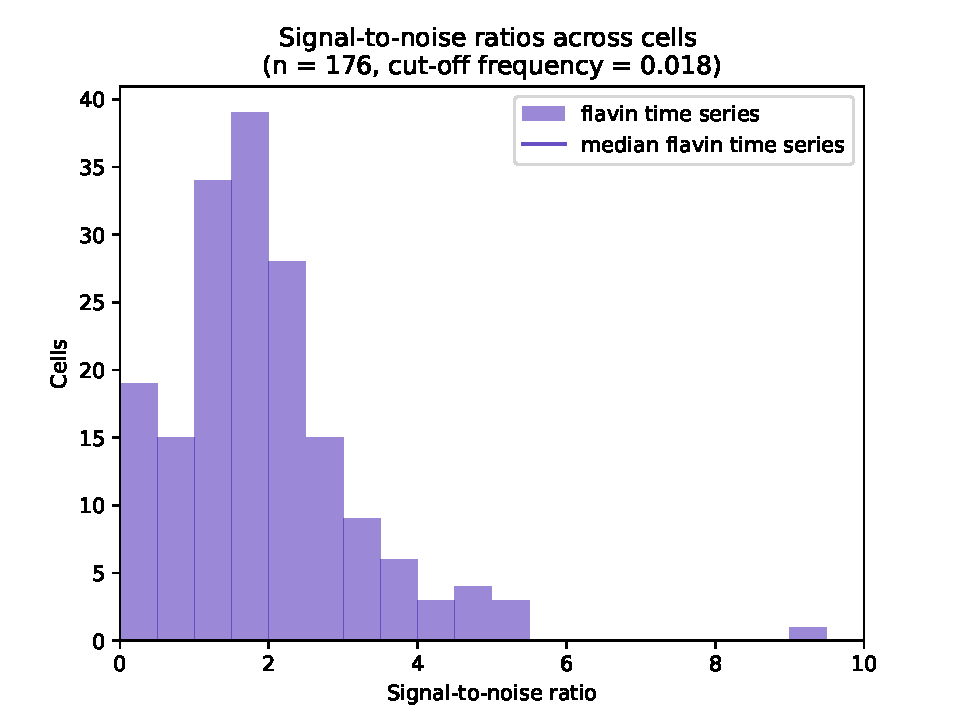
\includegraphics[width=.9\linewidth]{tsa1tsa2morgan_1253_plots_10.pdf}
\end{center} Subfigure X.X: Distribution of signal-to-noise ratios computed for each flavin time series derived from tsa1\(\Delta\) tsa2\(\Delta\) cells, showing a wide distribution of quality of oscillation.
\end{itemize}
\end{itemize}


\section{Discussion}
\label{sec:biology-discussion}

\subsection{Interpretation of results}
\label{subsec:biology-discussion-interpretation}
\begin{enumerate}
\item Presence of flavin-based single-cell metabolic cycles, which are autonomous and gate the cell division cycle.
\begin{itemize}
\item Results confirm \cite{papagiannakisAutonomousMetabolicOscillations2017} and \cite{baumgartnerFlavinbasedMetabolicCycles2018}.  In high glucose, flavin cycles are asynchronous between cells and peaks in flavin fluorescence coincide with bud formation.
\begin{itemize}
\item We expect the flavin fluorescence to peak when buds form, and this is our reasoning:
\begin{itemize}
\item NAD(P)H fluorescence peaks -- i.e. the molecule is in the reduced NAD(P)H form -- when buds form (\cite{papagiannakisAutonomousMetabolicOscillations2017}).  Flavins should be in the oxidised form when NAD(P)H is in the reduced form because the flavoprotein lipoamide dehydrogenase is in redox equilibrium with NAD(P)H (\cite{sianoNADHFlavinFluorescence1989}, and also confirmed by several reactions catalysed by \href{Flavoproteins.org}{Flavoproteins} (example proteins and citations needed).  Flavins fluoresce in the oxidised form, thus we expect flavin fluorescence to peak. \cite{murrayRedoxRegulationRespiring2011} confirms that flavin and NAD(P)H fluorescence to peak in phase in continuous chemostat cultures.
\end{itemize}

\begin{itemize}
\item It would be nice to support this logic with the roles of flavoproteins (\cite{gudipatiFlavoproteomeYeastSaccharomyces2014}).  However, it is difficult because we can't readily assume the behaviour of individual flavoproteins based on the behaviour of their aggregrate.
\end{itemize}
\end{itemize}
\item Results in pyruvate reveal that as the metabolic cycle lengthens, G1 lengthens but S/M stays the same length, reinforcing a model in which a specific phase of the metabolic cycle gates entry into the cell division cycle.  This is consistent with \cite{oneillEukaryoticCellBiology2020} and (add other citations here).
\item Cross-correlation between flavin and mCherry signals further confirm the sequence of events while the two biological oscillations (metabolic cycle \& cell division cycle) progress.  This is more obvious in pyruvate  Specifically, when the new bud forms, the mother cell's flavin fluorescence peaks.  Subsequently, the cell synthesises new histones in S phase, then the cell enters anaphase -- characterised by the sharp drop in the mCherry signal -- as the flavin fluorescence is at its trough.
\item Metabolic cycles still occur even when cells do not divide.  This holds true for 'one-off' skipping of cell division and conditions in which cells pause cell division for long periods of time.  My observations add to \cite{baumgartnerFlavinbasedMetabolicCycles2018} that stopped cell divisions using alpha-factor; I stopped them in a different way.
\item Confirms \cite{ozsezenInferenceHighLevelInteraction2019}.
\end{itemize}
\item Cells individually generate metabolic cycles and individually adapt them in response to nutrient changes.
\begin{itemize}
\item Literature disputes whether metabolic oscillations arise from interactions between cells or whether cells individually generate oscillations.
\item Even though the cells are physically separated in traps and nutrient media flows through them, single-cell flavin oscillations can synchronise and reset phase in certain conditions.  Diffusible metabolites cannot be responsible.  We thus conclude that each cell -- on its own -- can reset its metabolic cycle in response to nutrient changes.
\begin{itemize}
\item Discussion: back-of-the-envelope physics calculations to show that diffusion at the timescale relevant to the experiments cannot be responsible for cell-to-cell synchrony given the physical distance between the cells and the flow rate.
\item Biochemical interpretation for the cell division cycle: if starvation occurs before START, cell remain in pause; if starvation occurs after START, cells go into pause.  Cells stuck in M phase during starvation?
\item Biochemical interpretation for the metabolic cycle: What biochemical mechanism does the cell use to reset the phase of its metabolic cycle?  How does this fit in with my model of explaining how the cycle works and coordinates cellular events (metabolism \& nutrient mobilisation) with the environment?  Link to FBA?
\end{itemize}
\item Doesn't necessarily mean that cells \emph{cannot} communicate with each other, but communication is \emph{not required}.
\end{itemize}
\item Cells adapt their metabolic cycle to nutrient conditions (\cite{papagiannakisAutonomousMetabolicOscillations2017}, other citations may be useful)
\begin{itemize}
\item The behaviour of the metabolic cycle changes when the cells are grown on low glucose or on pyruvate.
\begin{itemize}
\item Biochemical interpretation: nutrient conditions that favour respiration over fermentation -- and thus slower growth rate -- leads to slower YMCs, but why?
\item Do the periods conform to those reported by \cite{papagiannakisAutonomousMetabolicOscillations2017}?  If not, why?
\end{itemize}
\end{itemize}
\item Reconciling chemostat and single-cell studies.

\begin{itemize}
\item In chemostats, glucose is limiting (\cite{jonesCyberneticModelGrowth1999}).  Synchrony of metabolic cycles between cells in respiring conditions may explain observations in chemostat as cells are near glucose starvation in these conditions.
\item Single-cell metabolic cycles in zwf1\(\Delta\) are inconsistent, and this may explain the absence of dissolved-oxygen oscillations in the chemostat.  zwf1\(\Delta\) affects many metabolic processes; most notably, it removes a major pathway of NAD(P)H generation from reduction of NAD(P)+.  The most abundant flavoproteins involve NAD(P)H redox, so it it reasonable to believe that flavin oscillations are affected.  Perhaps zwf1\(\Delta\) impairs the metabolic cycle in some way.
\item However, difference between single-cell and chemostat traces warrant a model to explain the differences.  Likely something to do with population.  Highlights weakness of chemostat experiments.
\begin{itemize}
\item See e.g. \cite{burnettiCellCycleStart2016}
\end{itemize}
\end{itemize}
\item Our analysis methods add on to those used in previous single-cell studies of the metabolic cycle.
\begin{itemize}
\item This is important because data processing steps can substantially alter the conclusions of any time series analysis study.
\item We pre-process the time series better.  Specifically, we use a Butterworth filter rather than sliding-window or Savitzky-Golay detrending so we have better control over the frequencies.
\item We use several analysis methods, some from the circadian rhythm literature, in conjunction with each other to confirm features of the oscillatory signals.  We use cross-correlation and Granger causality analysis to quantify the sequence of events in biological oscillators and these methods utilise more information than comparing peaks of time series as performed previously.
\end{itemize}
\end{enumerate}

\subsection{Broader implications}
\label{sec:biology-discussion-implications}

\begin{itemize}
\item Confirms utility of using flavin as an indicator of YMC.  Confirms utility of our microfluidics platform.  Our technology produces vast amounts of data, so our computational tools are especially useful.  Confirms utility of our analysis methods.
\item Confirms model in which autonomous, single-cell YMC responds to nutrient conditions and adjusts period/phase accordingly.  YMC-CDC synchrony holds in a window of frequencies -- outside this, YMCs still occur but coupling changes.  Points to model that YMCs govern cell resources and only if they are adequate does the cell initiate a CDC.  Suggestion that deletion strain impair this model.
\item Autonomy of YMCs (cell-autonomous and independence from CDC), starvation in chemostat, and presence of subpopulations may explain differences between chemostat and single-cell based studies.  My study makes the case for studying this system in single-cell as it gives more info than chemostat.
\item Something fundamental to control of biological rhythms?  Links to other processes?
\begin{itemize}
\item pH and growth rate oscillations (\cite{luziaPHDependenciesGlycolytic})
\end{itemize}
\end{itemize}
